\section{Durchführung}
\label{sec:Durchführung}
\renewcommand{\labelenumi}{\alph{enumi})}
\begin{enumerate}
%\begin{figure}[H]
%    \centering
%    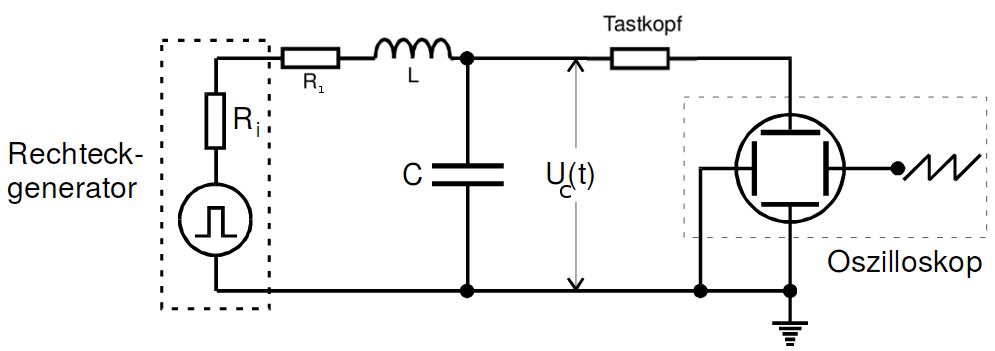
\includegraphics[width=\linewidth-200pt,height=\textheight-200pt,keepaspectratio]{content/Aufgabea.png}
%    \caption{Schaltung zur Bestimmung des effektiven Widerstandes aufgrund seiner Dämpfwirkung.}
%    \label{fig:Schaltplana}
%  \end{figure}
\item Es wird zunächst die Amplitude einer gedämpften Schwingung auf ihre Zeitabhängigkeit hin untersucht, indem
 der effektive Dämpfungswiderstand ermittelt wird. Hierzu wird ein $RCL$-Kreis gemäß
 Abb. 4  angeschlossen. Der Generator wird auf Rechteckimpulse gestellt.
  Die Generatorfrequenz wird so gewählt, dass die Schwingungsamplitude des $RCL$-Kreises auf etwa $\frac{1}{6}$
   ihres ursprünglichen Wertes gesunken ist, bevor sie einen neuen Impuls erfährt. Das Oszilloskop
    wird dementsprechend eingestellt, sodass der Schwingungsverlauf vollständig auf dem Bildschirm einsehbar ist.
    Anschließend wird ein Abbild des Bildschirm für die Auswertung angefertigt.
    %Für diese wird die Einhüllende der Schwingungskurve in das Abbild eingezeichnet.
     %Zusätzlich werden dem Graphen einige Wertepaare für eine logarithmische Ausgleichsrechnung entnommen.
      %Aus der bestimmten Steigung werden schließlich der effektive Widerstand $R_{eff}$ sowie die Abklingzeit $\tau$  mit (10) ermittelt.
       %Zudem soll $R_{eff}$ mit dem in der Schaltung verbauten R verglichen werden.

     \item Es soll der Dämpfungswiderstand $R_{ap}$ bestimmt werden, bei der der aperiodische Grenzfall des Systems vorliegt.
     Dazu wird der feste Widerstand durch einen variablen Widerstand $R_v$
     ausgetauscht. Dieser wird auf seinen Maximalwert eingestellt, sodass das System ein Relaxationverhalten zeigt.
      Anschließend verringert man $R_v$ solange, bis sich das Relaxationsverhalten hin zu einer Schwingung umformt.
      Hat man diesen Punkt erreicht, dreht man $R_v$ wieder etwas nach oben, bis der Graph keine Überschwinger mehr zeigt.
      %Für die Auswertung wird der gemessene $R_{ap}$-Wert mit dem aus L und C berechneten Theoriewert verglichen.
       %Dieser berechnet sich mit:
       %\begin{equation}
        % R_{ap} = 2\sqrt{\frac{L}{C}}
       %\end{equation}
%\begin{figure}[H]
         %\centering
         %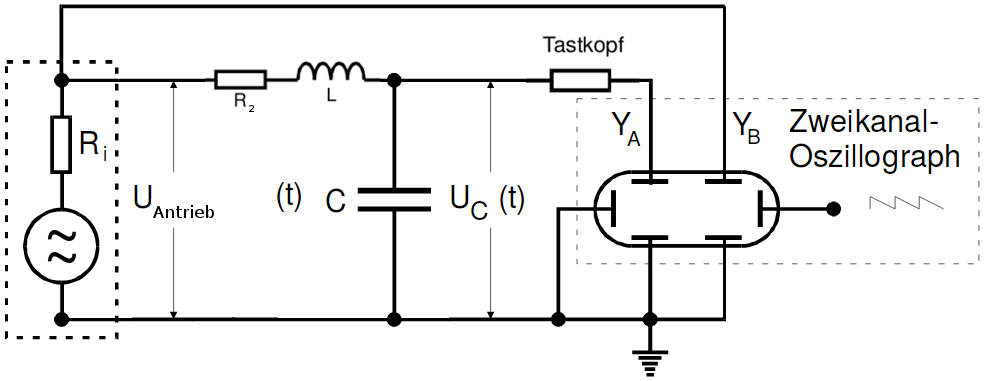
\includegraphics[width=\linewidth-200pt,height=\textheight-200pt,keepaspectratio]{content/Aufgabec.png}
         %\caption{Schaltung zur Untersuchung der Resonanzeffekte und Phasenverschiebung zwischen $A_C$ und $A_{Antrieb}$}
         %\label{fig:Schalplanc}
       %\end{figure}
      \item Es wird ein in Reihe geschalteter $RCL$-Kreis auf die Frequenzabhängigkeit seiner Kondensatorspannung hin untersucht.
      Hierzu wird zusätzlich die Antriebsspannung direkt über den zweiten Kanal an das Oszilloskop angeschlossen. Der Funktionsgenerator wird auf eine Sinusspannung eingestellt.
      Anschließend wird eine Messreihe von $U_C$ für verschiedene Frequenzen durchgeführt.
       Da auch die Amplitude $A_{\text{Antrieb}}$ der Ausgangsspannung $U_{\text{Antrieb}}$ am Tastkopf frequenzabhängig ist, ist es notwendig, diese mitzunotieren.
       %Zur Auswertung wird $\frac{A_C}{A_{Antrieb}}$ gegen $f_{Antrieb}$ in ein halblogarithmisches Diagramm eingetragen. Anhand von diesem wird
        %anschließend die Güte q bestimmt.Der Bereich um die Resonanzfrequenz $f_{res}$ soll zudem nochmals linear
         %abgebildet werden. Hieraus wird zusätzlich die Breite der Resonanzkurve ermittelt.
         %Anschließend werden die Ergebnisse mit den errechneten Theoriewerten nach (16) und (17) verglichen.

         \item Zuletzt wird die Frequenzabhängigkeit der Phase zwischen $U_C$ und $U_{Antrieb}$ des
          $RCL$-Kreises untersucht. Auch hier wird zusätzlich die Antriebsspannung direkt über das Oszilloskop ausgegeben.
          angeschlossen. Das Oszilloskop wird so eingestellt, sodass die Graphen von $U_C$ und $U_{Antrieb}$ übereinander liegen.
             Anschließend werden jeweils
      $\Delta t$ zwischen den Nullstellen und die zugehörige Frequenz notiert. Die jeweilige
       Phasendifferenz berechnet sich mit:
       \begin{equation}
         \varphi = 2 \pi \cdot \Delta t \cdot f_{Antrieb}
       \end{equation}
      % Für die Auswertung wird $\varphi$ gegenüber f in einem halblogarithmischen
      %  Diagramm aufgetragen. Der Bereich um $\varphi = \frac{\pi}{2}$ wird zusätzlich
      %   linear dargestellt. Aus ihm entnimmt man $f_{res}$, $f_1$ und $f_2$,
      %    die $\omega_{res}$, $\omega_1$ und $\omega_2$ geteilt durch $2\pi$ entsprechen.
      %     Auch diese werden wieder
      %   mit den nach (19) berechneten verglichen.
\end{enumerate}
